% !TeX root = RJwrapper.tex
\title{Smooth Operator: Modifying the Anhøj Rules to Improve Runs Analysis in
Statistical Process Control}
\author{by Jacob Anhøj, Tore Wentzel-Larsen}

\maketitle

\abstract{%
The run charts is one form of statistical process control charts that is
particularly useful for detecting minor to moderate shifts in data over
time. The Anhøj rules test for shifts by looking for unusually long runs
(L) of data points on the same side of the process centre (mean or
median) and unusually few crossings (C) of the centre. The critical
values for C and L depend on the number of available data points (N).
Consequently, the diagnostic properties (e.g.~sensitivity and
specificity) of the Anhøj rules also depend on N and have a rugged
appearance due to the discrete nature of the tests. This study
demonstrates that it is possible to obtain better diagnostic properties
by making minor adjustment to the critical values for C and L. We refer
to these procedures as the best box and cut box adjustment procedures.
}

% Any extra LaTeX you need in the preamble

\hypertarget{introduction}{%
\subsection{Introduction}\label{introduction}}

Within statistical process control (SPC) runs analysis is being used to
detect persistent shifts in process location over time
\citep{anhoej2018}.

Runs analysis deals with the natural limits of number of runs and run
lengths in random processes. A run is a series of one or more
consecutive elements of the same kind, for example heads and tails,
diseased and non-diseased individuals, or numbers above or below a
certain value. A run chart is a point-and-line chart showing data over
time with the median as reference line (Figure \ref{figure:run}). In a
random process, the data points will be randomly distributed around the
median, and the number and lengths of runs will be predictable within
limits. All things being equal, if the process shifts, runs tend to
become longer and fewer. Consequently, runs analysis may help detect
shifts in process location. Process shifts are one form of non-random
variation in time series data that are of particular interest to quality
control and improvement: If a process shifts, it may be the result of
planned improvement or unwanted deterioration.

\begin{figure}[htbp]
  \centering
  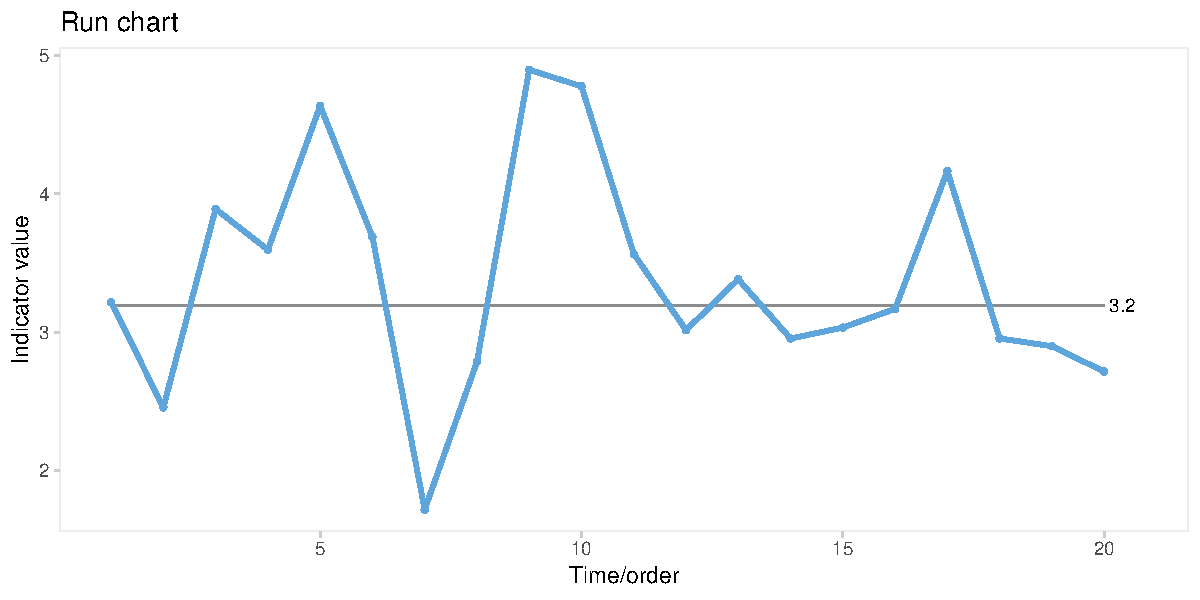
\includegraphics[width=\textwidth]{fig_run.pdf}
  \caption{Run chart. Median = 3.2, longest run (L) = 4, number of crossings (C) = 9.}
  \label{figure:run}
\end{figure}

Several tests (or rules) based on the principles of runs analysis for
detection of shifts exist. In previous papers we demonstrated, using
simulated data series, that the currently best performing rules with
respect to sensitivity and specificity to shifts in process location are
two simple tests \citep{anhoej2014, anhoej2015, anhoej2018}:

\begin{itemize}
\item
  Shifts test: one or more unusually long runs of data points on the
  same side of the centre line.
\item
  Crossings test: the curve crosses the centre line unusually few times.
\end{itemize}

Collectively, we refer to these tests as the Anhøj rules, which are the
default rules used for run and control chart analysis with the
\CRANpkg{qicharts2} package \citep{qicharts2}. For a thorough discussion
of the practical use of run and control charts for quality improvement
we refer to the \CRANpkg{qicharts2} package vignette.

Critical values for run length and number of crossings depend on the
total number of data points in the chart. The number of crossings follow
a binomial distribution, \(b(n - 1, 0.5)\), where n is the number of
data points and 0.5 the success probability. Thus, the lower prediction
limit for number of crossings may, for example, be set to the lower 5th
percentile of the corresponding cumulative binomial distribution
\citep{chen2010}. However, no closed form expression exists for the
distribution of longest runs. Consequently, the upper prediction limit
for longest runs has traditionally been either a fixed value (usually 7
or 8) \citep{carey2002a} or an approximate value depending on n as with
the Anhøj rules: \(\log_2(n) + 3\) rounded to the nearest integer
\citep{schilling2012}. Figure \ref{figure:run} has 20 data points, the
curve crosses the centre line 9 times, and the longest run (points 3-6)
contains 4 data points. In a random process with 20 data points, we
should expect at least 6 crossings and the longest run should include no
more than 7 data points. Thus, according to the Anhøj rules, Figure
\ref{figure:run} shows random variation.

Each of the two tests has an overall specificity (true negative
proportion) around 95\%. The sensitivity (true positive proportion) of a
test depends on the size of the shift (signal) relative to the random
variation inherent in the process (noise). When applied together, the
sensitivity increases, while the specificity decreases a bit and
fluctuates around 92.5\% (see red line in Figure \ref{figure:spec}).

\begin{figure}[htbp]
  \centering
  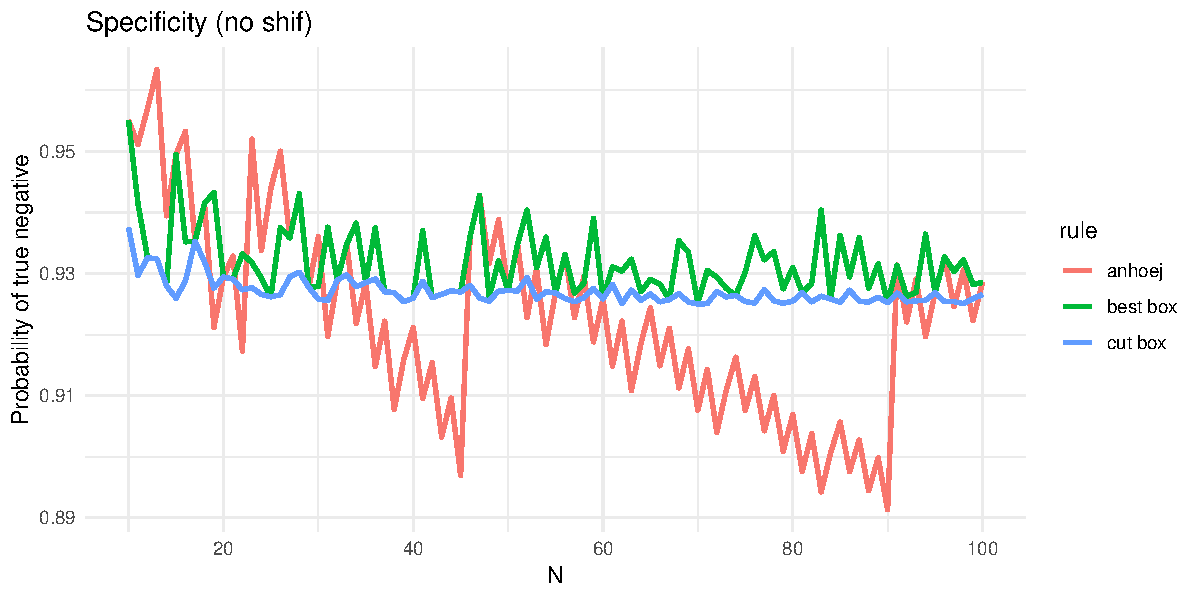
\includegraphics[width=\textwidth]{fig_spec.pdf}
  \caption{Specificity of the Anhøj, best box, and cut box rules. N = number of data points in run chart. }
  \label{figure:spec}
\end{figure}

Historically, runs tests have mainly been studied individually. But what
is really of interest, because the rules are linked -- when one goes up,
the other goes down -- is the properties of the joint distribution of
number of crossings (C) and longest runs (L).

We recently released an R package, \CRANpkg{crossrun} \citep{twl2018},
that includes functions for calculating the joint probabilities of C and
L in random data series of different lengths (N) and with and without
shifts in process location expressed in standard deviation units (SD).
Figure \ref{figure:box11} illustrates this for a run chart with N = 11
and SD = 0 (no shift). To avoid very small numbers, the probabilities
are shown using the times representation, that is, the probabilities
times \(2^{n-1}\), which is 1024 for N = 11. The red box encloses the
combinations of C and L that would indicate random variation according
to the Anhøj rules (true negatives). The area outside the box represents
combinations of C and L that would indicate non-random variation (false
positives).

\begin{figure}[htbp]
  \centering
  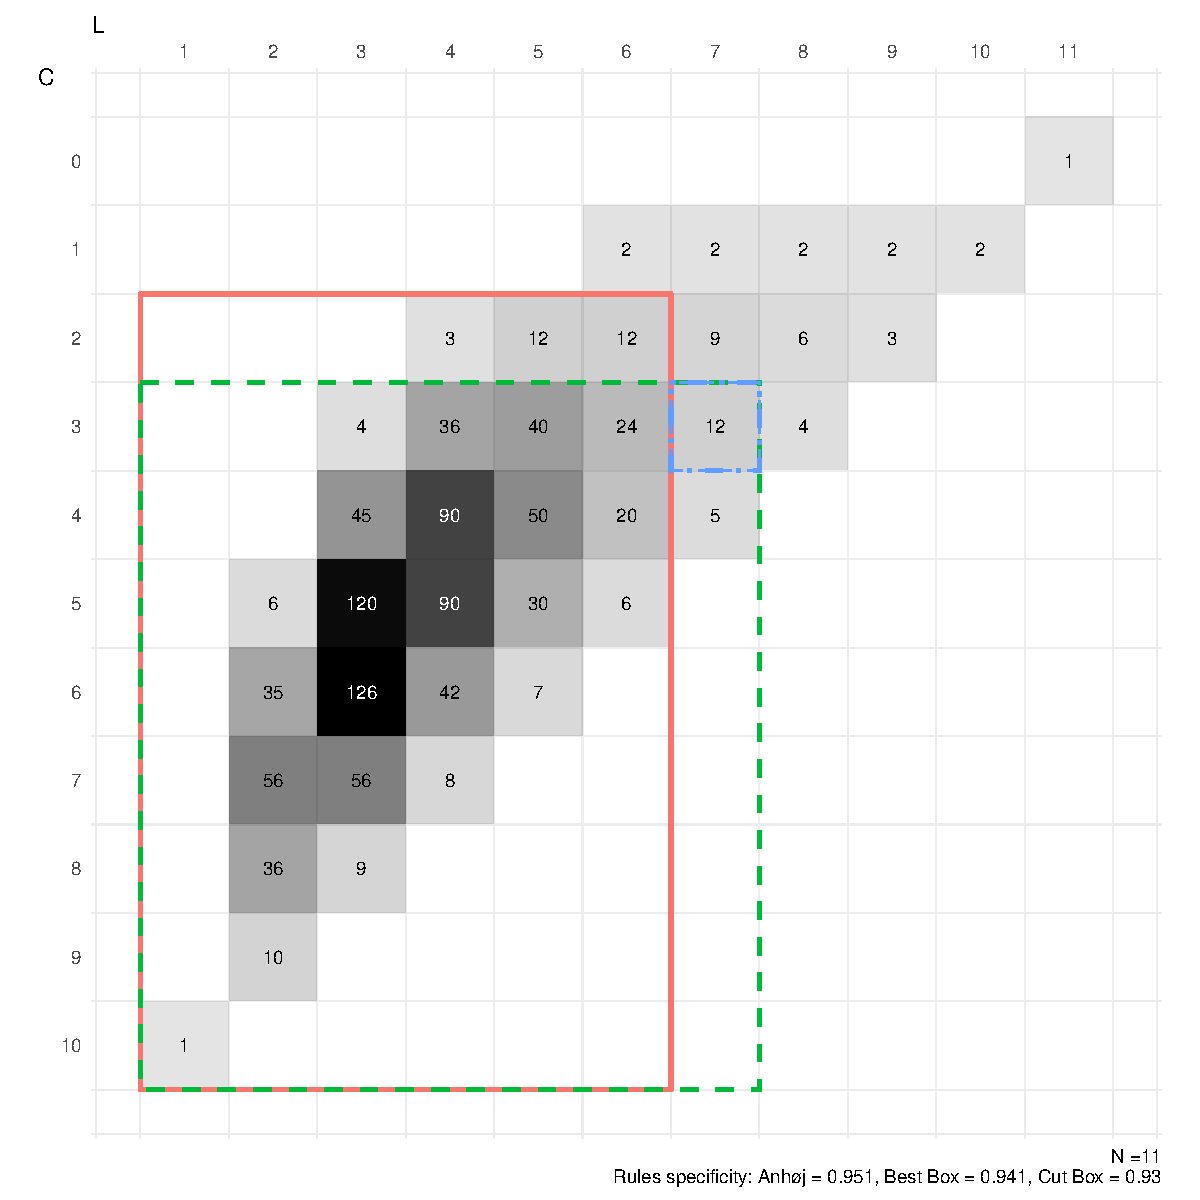
\includegraphics[width=\textwidth]{fig_box11.pdf}
  \caption{Borders of the Anhøj, best box, and cut box rules for N = 11 data points. 
           C = number of crossings, L = longest run.
           The numbers in the cells are times representation of of the joint
           probabilities of longest run and number of crossings.
           Anhøj = red solid, best box = green dashed, cut box = blue dot-dashed.}
  \label{figure:box11}
\end{figure}

With the \CRANpkg{crossrun} package it became feasible to calculate
exact joint probabilities of C and L over a wide range of N and SD. And
consequently, it became feasible to investigate the diagnostic
properties of run charts using exact values for specificity and
sensitivity rather than values based on time consuming, inaccurate, and
complicated simulation studies.

As shown in Figure \ref{figure:spec} the specificity of the Anhøj rules
(red line) jumps up and down as N changes. This is a consequence of the
discrete nature of the two tests -- especially the shifts test. Although
the specificity of the Anhøj rules does not decrease continuously as N
increases, which is the case for other rules \citep{anhoej2014}, we
hypothesised that it would be possible to improve the diagnostic value
further by smoothing the specificity using minor adjustments to C and L
depending on N.

The aims of this study were to provide exact values for the diagnostic
properties of the Anhøj rules and to suggest a ``smoothing'' procedure
for improving the value of runs analysis.

\hypertarget{methods}{%
\subsection{Methods}\label{methods}}

\hypertarget{likelihood-ratios-to-quantify-the-diagnostic-value-of-runs-rules}{%
\subsubsection{Likelihood ratios to quantify the diagnostic value of
runs
rules}\label{likelihood-ratios-to-quantify-the-diagnostic-value-of-runs-rules}}

The value of a diagnostic test is traditionally described using terms
like sensitivity and specificity. These parameters express the
probability of detecting the condition being tested for when it is
present and not detecting it when it is absent:

\[ \text{Specificity = P(no signal | no shift) = P(true negative) = 1} - \text{P(false positive)} \]
\[ \text{Sensitivity = P(signal | shift) = P(true positive) = 1} - \text{P(false negative)} \]

However, we usually seek to answer the opposite question: what is the
likelihood that a positive or negative test actually represents the
condition being tested for, which in our case is a shift in the
underlying process? Likelihood ratios (LR) do this:

\[ \text{LR+ = TP/FP = sensitivity/(1} - \text{specificity)} \]
\[ \text{LR- = FN/TN = (1} - \text{sensitivity)/specificity} \]

A likelihood ratio greater than 1 speaks in favour of the condition
being tested for, while a likelihood ratio less than 1 speaks against
the condition. As a rule of thumb, a positive likelihood ratio (LR+)
greater than 10 is considered strong evidence that the condition is
present. A negative likelihood ratio (LR-) smaller than 0.1 is
considered strong evidence against the condition \citep{deeks2004}. For
example, if LR+ = 10 and LR- = 0.1 then a positive test means that it is
10 times \emph{more} likely that the condition is present than not
present, and a negative test means that it is 10 times \emph{less}
likely that the condition is present than not present. Thus, likelihood
ratios come in pairs and are combined measures of the usefulness of a
diagnostic test. Specifically, for our purpose, runs charts are
diagnostic test for non-random variation in time series data
\citep{anhoej2015, anhoej2018}.

\hypertarget{best-box-and-cut-box-adjustments-to-improve-the-anhj-rules}{%
\subsubsection{Best box and cut box adjustments to improve the Anhøj
rules}\label{best-box-and-cut-box-adjustments-to-improve-the-anhj-rules}}

To fix some terms, we define a box as a square region
\(C \geq c, L \leq l\). These are the square regions that may be used to
define random variation. The corner of the box is its upper right square
\(C = c, L = l\). In Figure \ref{figure:box11} the box
\(C \geq 2, L \leq 6\), marked with red, specifies the Anhøj rules for
\(N=11\). The corner of this box is the square \(C = 2, L = 6\).

Based on the \CRANpkg{crossrun} package we developed two functions,
\code{bestbox()} and \code{cutbox()} that automatically seek to adjust
the critical values for C and L to balance between sensitivity and
specificity requirements. Specifically, the \code{bestbox()} function
finds the box with highest sensitivity for a pre-determined shift (the
target shift), among boxes with specificity \(\geq\) a pre-determined
value (the target specificity). The \code{cutbox()} function
subsequently cuts squares from the upper and right borders of the best
box, starting from the corner while keeping specificity \(\geq\) its
target value, and the sensitivity for the target shift as large as
possible. The result of \code{cutbox()} is not necessarily a box, but a
reasonable region for declaring random variation with one or a few
squares close to the corner possibly removed.

In this study we used a target specificity of 92.5\%, which is close to
the actual average specificity for the Anhøj rules for N = 10-100, while
the target shift was set at 0.8.

Figure \ref{figure:box11} illustrates these principles for a run chart
with 11 data points. Thus, for N = 11, the Anhøj rules would signal a
shift if C \textless{} 2 or L \textgreater{} 6; best box would signal if
C \textless{} 3 or L \textgreater{} 7; and cut box would signal if C
\textless{} 3 or L \textgreater{} 7, and also when C = 3 and L = 7.

\hypertarget{results}{%
\subsection{Results}\label{results}}

We calculated the limits for the Anhøj, best box, and cut box rules
together with their corresponding positive test proportions and
log-likelihood ratios for N = 10-100 and SD = 0-3 (in 0.2 SD
increments). We stored the \code{log} of likelihood ratios to preserve
numerical precision. To get the actual likelihood values back, use
\code{exp(log-likelihood)}. The limits, specificities, and sensitivities
are presented in Table \ref{tab:tab1}. The R code to reproduce the full
results set and the figures from this article is provided in the
supplementary file \file{crossrunbox.R}.

Figure \ref{figure:spec} illustrates the effect of the best box and cut
box procedures on the specificity of the runs analysis. As expected, the
variability in specificity with varying N is markedly reduced and kept
above and closer to the specified target -- more with cut box than with
best box.

Figure \ref{figure:pwr} shows the probabilities of getting a signal as a
function of N and SD. The upper left facet (SD = 0) contains the same
data as Figure \ref{figure:spec}. As expected and shown previously in
our simulation studies, the power of the runs analysis increases with
increasing N and SD. The smoothing effect of best box and cut box
appears to wear off as N and SD increases. Figure \ref{figure:sens} is a
blown up version of the facet with shift = 0.8 SD from Figure
\ref{figure:pwr} and shows the sensitivity for the target value used in
the box calculations. Exact values for shift = 0 and shift = 0.8 may be
looked up in Table \ref{tab:tab1}

\begin{figure}[htbp]
  \centering
  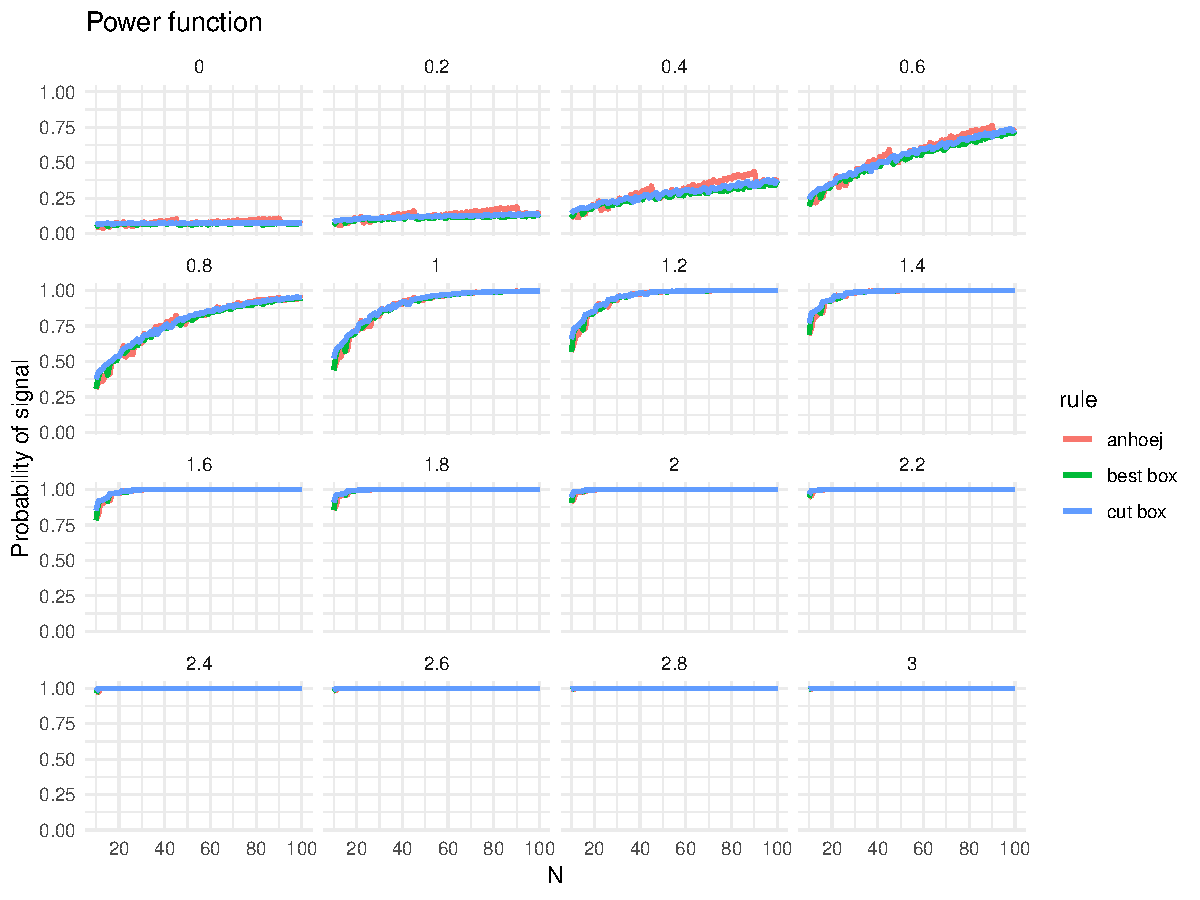
\includegraphics[width=\textwidth]{fig_pwr.pdf}
  \caption{Power function of Anhøj, best box, and cut box rules.
           N = number of data points in run chart.
           Numbers above each facet represent the size of the shift in standard
           deviation units (SD) that is present in data.}
  \label{figure:pwr}
\end{figure}

\begin{figure}[htbp]
  \centering
  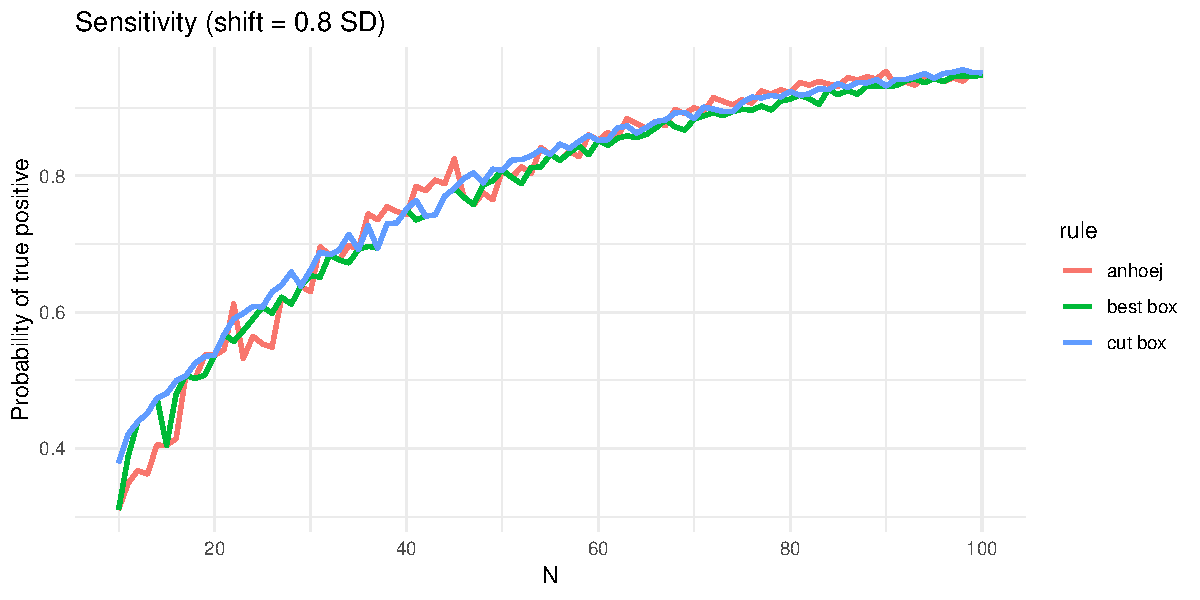
\includegraphics[width=\textwidth]{fig_sens.pdf}
  \caption{Sensitivity of Anhøj, best box, and cut box rules for shift = 0.8
           standard deviation units.
           N = number of data points in run chart.}
  \label{figure:sens}
\end{figure}

Figures \ref{figure:lrpos} and \ref{figure:lrneg} compare the positive
and negative likelihood ratios of the Anhøj rules to the box
adjustments. The smoothing effect appear to be of practical value only
for positive tests.

\begin{figure}[htbp]
  \centering
  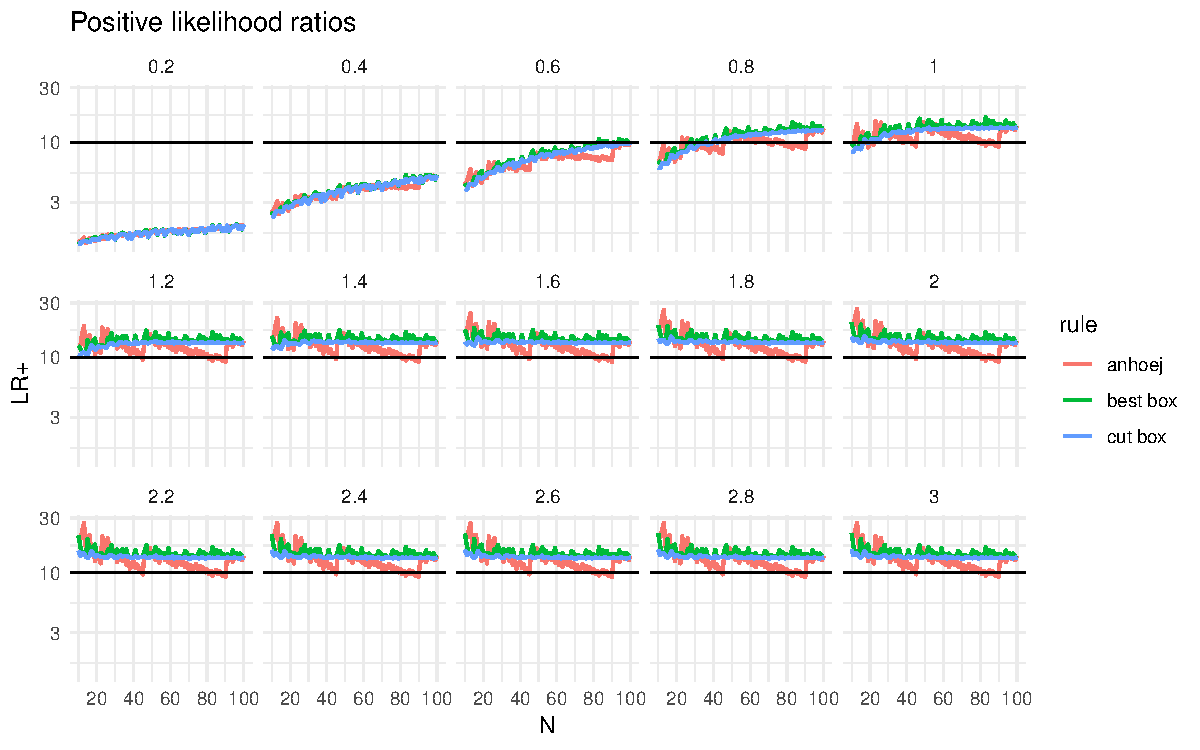
\includegraphics[width=\textwidth]{fig_lrpos.pdf}
  \caption{Positive likelihood ratio of Anhøj, best box, and cut box rules.
           N = number of data points in run chart.
           Numbers above each facet represent the size of the shift in standard
           deviation units that is present in data.}
  \label{figure:lrpos}
\end{figure}

\begin{figure}[htbp]
  \centering
  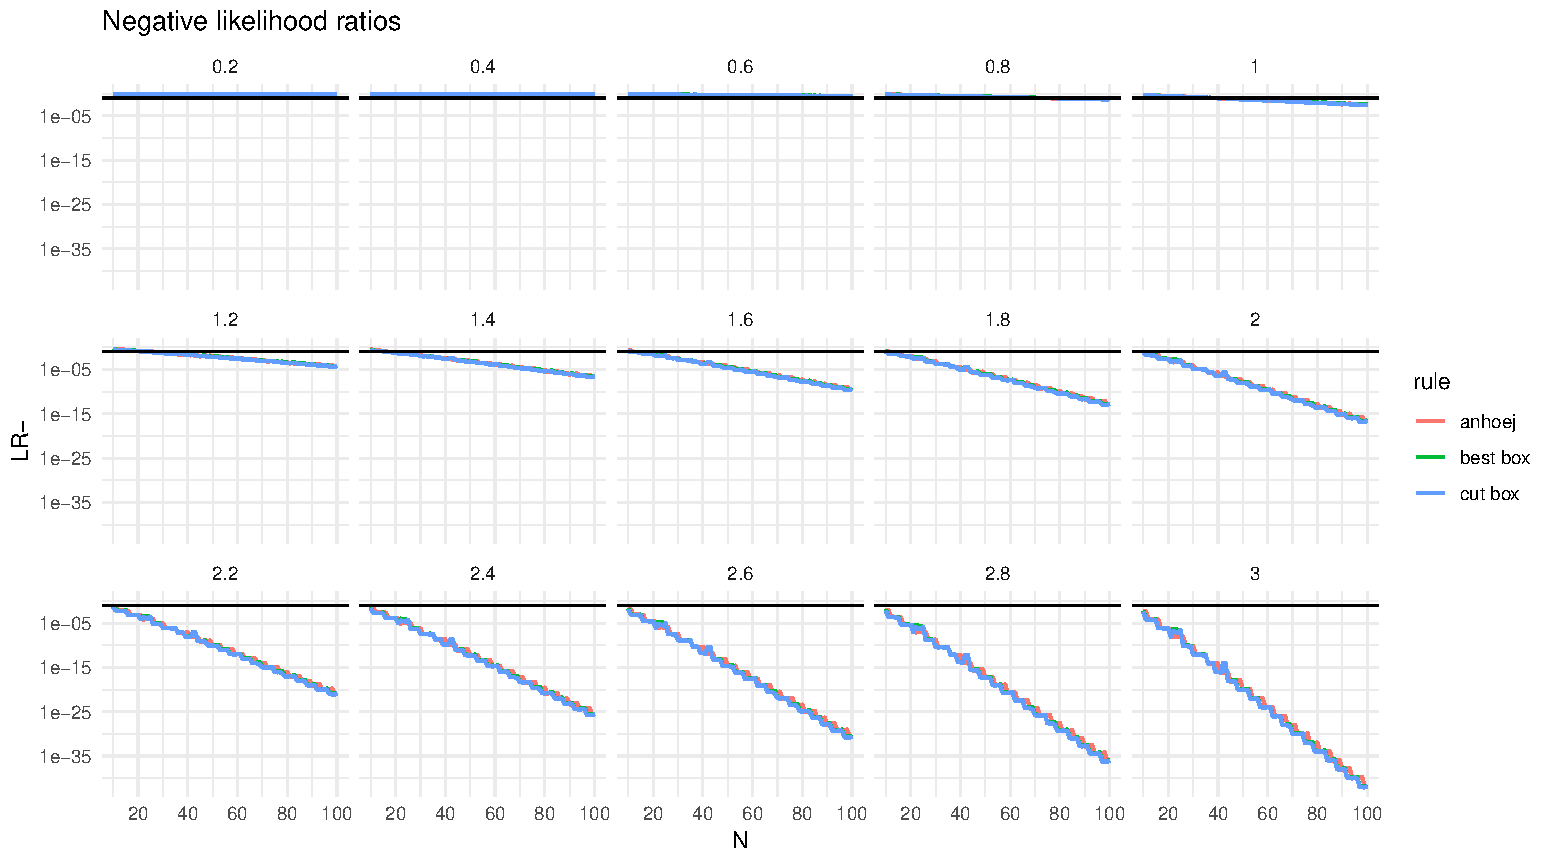
\includegraphics[width=\textwidth]{fig_lrneg.pdf}
  \caption{Negative likelihood ratio of Anhøj, best box, and cut box rules.
           N = number of data points in run chart.
           Numbers above each facet represent the size of the shift in standard
           deviation units (SD) that is present in data.}
  \label{figure:lrneg}
\end{figure}

\hypertarget{discussion-and-conclusion}{%
\subsection{Discussion and conclusion}\label{discussion-and-conclusion}}

This study provided exact values for the diagnostic properties of the
Anhøj rules for run charts with 10-100 data points including shifts up
to 3 standard deviation units.

To our knowledge, and with the exception of our own \CRANpkg{crossrun}
package, the properties of the joint distribution of number of crossings
and longest runs in random data series have not been studied before.

Furthermore, the study demonstrated that it is feasible to reduce the
variability in run chart specificity with varying number of data points
by using the best box and cut box adjustments of the Anhøj rules.

Most importantly, figures \ref{figure:lrpos} and \ref{figure:lrneg}
confirm what we expected after years of practical experience using runs
analysis, that the Anhøj rules is a useful and robust method for
detection of persistent shifts only slightly larger than 1 standard
deviation units and with as little as 10-12 data points. This can be
seen by the fact that LR+ \textgreater{} 10 for SD \textgreater{} 1 and
N \(\geq\) 10. Although, the best box and cut box procedures will not
change this, the box adjustments may potentially improve the practical
value of runs analysis by reducing sudden shifts in sensitivity and
specificity when the number of available data points changes. Whether
this holds true in practice remains to be confirmed.

The study has two important limitations. First, the calculations of box
probabilities require that the process centre is fixed and known in
advance, for example, the median from historical data. In practice the
centre line is often determined from the actual data in the run chart,
in which case the calculations of box probabilities do not apply.
Preliminary studies suggest that this is mostly relevant for short data
series. We plan to include a function in a future update of
\CRANpkg{crossrun} to calculate the box probabilities with empirical
centre lines.

Second, the procedures have so far only been checked for up to 100 data
points. Because of the iterative procedures and use of high precision
numbers using functions from the \CRANpkg{Rmpfr} package \citep{rmpfr}
to calculate the joint distributions for varying N, the computations are
time consuming. On a laptop with an Intel Core i5 processor and 8 GB
RAM, it takes about one hour to complete \code{crossrunbox.R} for N =
10-100 and SD = 0-3, and the objects created consume over 6 GB of
memory. However, we have no reason to believe that the procedures are
not valid for N \textgreater{} 100, but the application of the box
procedures for larger N may be impractical at the moment.

Also, one should be aware that the value of the box procedures rely on
the choice of target specificity and target shift values. Other target
values will give different diagnostic properties. Preliminary studies
suggest that increasing the target specificity to, say, 0.95 in fact
increases the positive likelihood ratios a bit without affecting the
negative likehood ratios considerably. By supplying the R code, we
encourage users to adapt our findings to their own needs.

Regarding the practical application of the box adjustment of the Anhøj
rules, we are in the process of testing a \code{method} argument for the
\code{qic()} function from the \CRANpkg{qicharts2} package that allows
the user to choose between \code{"anhoej"}, \code{"bestbox"}, and
\code{"cutbox"} methods to identify non-random variation in run and
control charts with up to 100 data points. This will allow us and others
to quickly gain practical experience with box adjustments on real life
data.

In conclusion, this study provided exact values for the diagnostic
properties of the Anhøj rules for run charts with 10-100 data points
including shifts up to 3 standard deviation units, and demonstrated that
it is feasible to reduce the variability in run chart specificity from
varying numbers of data points by using the best box and cut box
adjustments of the Anhøj rules.

\bibliography{RJreferences}

\newpage

\hypertarget{appendix-results-table}{%
\subsection{Appendix: Results table}\label{appendix-results-table}}

\begin{Schunk}

\begin{longtable}{rrrrrrrrrrrrr}
\caption{\label{tab:tab1}Signal limits, specificity, and sensitivity for the Anhøj and best box
        rules and borders for the cut box rules. N = number of data points in
        chart.
        C = lower limit for number of crossings, L = upper limit for longest 
        run,  for declaring random variation by the Anhøj and best box rules. 
        Cbord and Lbord = Additional information for the cut box rules. When
        specified, parts of the border of the best box to retain to declare
        random variation. When not specified, cut box is identical to best box.}\\
\toprule
\multicolumn{1}{c}{ } & \multicolumn{2}{c}{Anhøj} & \multicolumn{2}{c}{Best box} & \multicolumn{2}{c}{Cut box} & \multicolumn{3}{c}{Specificity, shift = 0.0 SD} & \multicolumn{3}{c}{Sensitivity, shift = 0.8 SD} \\
\cmidrule(l{3pt}r{3pt}){2-3} \cmidrule(l{3pt}r{3pt}){4-5} \cmidrule(l{3pt}r{3pt}){6-7} \cmidrule(l{3pt}r{3pt}){8-10} \cmidrule(l{3pt}r{3pt}){11-13}
N & C & L & C & L & Cbord & Lbord & Anhøj & Best box & Cut box & Anhøj & Best box & Cut box\\
\midrule
\endfirsthead
\caption[]{Signal limits, specificity, and sensitivity for the Anhøj and best  \textit{(continued)}}\\
\toprule
\multicolumn{1}{c}{ } & \multicolumn{2}{c}{Anhøj} & \multicolumn{2}{c}{Best box} & \multicolumn{2}{c}{Cut box} & \multicolumn{3}{c}{Specificity, shift = 0.0 SD} & \multicolumn{3}{c}{Sensitivity, shift = 0.8 SD} \\
\cmidrule(l{3pt}r{3pt}){2-3} \cmidrule(l{3pt}r{3pt}){4-5} \cmidrule(l{3pt}r{3pt}){6-7} \cmidrule(l{3pt}r{3pt}){8-10} \cmidrule(l{3pt}r{3pt}){11-13}
N & C & L & C & L & Cbord & Lbord & Anhøj & Best box & Cut box & Anhøj & Best box & Cut box\\
\midrule
\endhead
\
\endfoot
\bottomrule
\endlastfoot
10 & 2 & 6 & 2 & 6 & 3 & 5 & 0.9551 & 0.9551 & 0.9375 & 0.3103 & 0.3103 & 0.3786\\
11 & 2 & 6 & 3 & 7 & 4 & 6 & 0.9512 & 0.9414 & 0.9297 & 0.3493 & 0.3887 & 0.4211\\
12 & 3 & 7 & 3 & 6 &  &  & 0.9570 & 0.9326 & 0.9326 & 0.3677 & 0.4392 & 0.4392\\
13 & 3 & 7 & 3 & 6 &  &  & 0.9634 & 0.9324 & 0.9324 & 0.3628 & 0.4519 & 0.4519\\
14 & 4 & 7 & 3 & 6 &  &  & 0.9395 & 0.9280 & 0.9280 & 0.4051 & 0.4740 & 0.4740\\
\addlinespace
15 & 4 & 7 & 4 & 7 & 6 & 6 & 0.9495 & 0.9495 & 0.9260 & 0.4046 & 0.4046 & 0.4806\\
16 & 4 & 7 & 5 & 8 & 6 & 7 & 0.9533 & 0.9352 & 0.9288 & 0.4146 & 0.4800 & 0.4993\\
17 & 5 & 7 & 5 & 7 &  &  & 0.9353 & 0.9353 & 0.9353 & 0.5069 & 0.5069 & 0.5069\\
18 & 5 & 7 & 5 & 7 & 6 & 6 & 0.9415 & 0.9415 & 0.9320 & 0.5030 & 0.5030 & 0.5256\\
19 & 6 & 7 & 5 & 7 & 6 & 5 & 0.9212 & 0.9433 & 0.9276 & 0.5370 & 0.5078 & 0.5351\\
\addlinespace
20 & 6 & 7 & 6 & 7 &  &  & 0.9294 & 0.9294 & 0.9294 & 0.5372 & 0.5372 & 0.5372\\
21 & 6 & 7 & 7 & 8 &  &  & 0.9328 & 0.9291 & 0.9291 & 0.5447 & 0.5672 & 0.5672\\
22 & 7 & 7 & 6 & 7 & 7 & 6 & 0.9173 & 0.9332 & 0.9273 & 0.6121 & 0.5573 & 0.5902\\
23 & 7 & 8 & 6 & 7 & 7 & 6 & 0.9520 & 0.9318 & 0.9277 & 0.5322 & 0.5728 & 0.5983\\
24 & 8 & 8 & 6 & 7 & 7 & 6 & 0.9338 & 0.9293 & 0.9266 & 0.5646 & 0.5900 & 0.6084\\
\addlinespace
25 & 8 & 8 & 6 & 7 &  &  & 0.9439 & 0.9262 & 0.9262 & 0.5536 & 0.6077 & 0.6077\\
26 & 8 & 8 & 9 & 9 & 10 & 7 & 0.9500 & 0.9375 & 0.9265 & 0.5488 & 0.5986 & 0.6298\\
27 & 9 & 8 & 9 & 8 & 10 & 7 & 0.9358 & 0.9358 & 0.9295 & 0.6221 & 0.6221 & 0.6397\\
28 & 9 & 8 & 9 & 8 & 11 & 7 & 0.9431 & 0.9431 & 0.9302 & 0.6118 & 0.6118 & 0.6589\\
29 & 10 & 8 & 10 & 8 &  &  & 0.9277 & 0.9277 & 0.9277 & 0.6382 & 0.6382 & 0.6382\\
\addlinespace
30 & 10 & 8 & 11 & 10 & 12 & 9 & 0.9360 & 0.9279 & 0.9258 & 0.6299 & 0.6533 & 0.6617\\
31 & 11 & 8 & 11 & 9 & 14 & 8 & 0.9197 & 0.9376 & 0.9256 & 0.6958 & 0.6515 & 0.6880\\
32 & 11 & 8 & 11 & 8 &  &  & 0.9289 & 0.9289 & 0.9289 & 0.6843 & 0.6843 & 0.6843\\
33 & 11 & 8 & 11 & 8 & 12 & 7 & 0.9348 & 0.9348 & 0.9298 & 0.6766 & 0.6766 & 0.6912\\
34 & 12 & 8 & 11 & 8 & 13 & 7 & 0.9218 & 0.9382 & 0.9278 & 0.6982 & 0.6724 & 0.7141\\
\addlinespace
35 & 12 & 8 & 12 & 8 &  &  & 0.9285 & 0.9285 & 0.9285 & 0.6920 & 0.6920 & 0.6920\\
36 & 13 & 8 & 13 & 9 & 15 & 8 & 0.9148 & 0.9375 & 0.9291 & 0.7442 & 0.6966 & 0.7265\\
37 & 13 & 8 & 14 & 10 &  &  & 0.9222 & 0.9270 & 0.9270 & 0.7356 & 0.6940 & 0.6940\\
38 & 14 & 8 & 13 & 8 &  &  & 0.9078 & 0.9269 & 0.9269 & 0.7548 & 0.7298 & 0.7298\\
39 & 14 & 8 & 15 & 11 &  &  & 0.9158 & 0.9254 & 0.9254 & 0.7475 & 0.7308 & 0.7308\\
\addlinespace
40 & 14 & 8 & 15 & 9 &  &  & 0.9212 & 0.9260 & 0.9260 & 0.7430 & 0.7509 & 0.7509\\
41 & 15 & 8 & 15 & 9 & 17 & 8 & 0.9095 & 0.9370 & 0.9287 & 0.7846 & 0.7353 & 0.7642\\
42 & 15 & 8 & 14 & 8 &  &  & 0.9154 & 0.9260 & 0.9260 & 0.7782 & 0.7408 & 0.7408\\
43 & 16 & 8 & 14 & 8 &  &  & 0.9032 & 0.9266 & 0.9266 & 0.7938 & 0.7427 & 0.7427\\
44 & 16 & 8 & 17 & 10 &  &  & 0.9096 & 0.9272 & 0.9272 & 0.7884 & 0.7704 & 0.7704\\
\addlinespace
45 & 17 & 8 & 17 & 9 &  &  & 0.8969 & 0.9270 & 0.9270 & 0.8249 & 0.7815 & 0.7815\\
46 & 17 & 9 & 17 & 9 & 19 & 8 & 0.9361 & 0.9361 & 0.9281 & 0.7687 & 0.7687 & 0.7961\\
47 & 17 & 9 & 17 & 9 & 20 & 7 & 0.9428 & 0.9428 & 0.9260 & 0.7576 & 0.7576 & 0.8045\\
48 & 18 & 9 & 19 & 12 & 20 & 11 & 0.9317 & 0.9261 & 0.9255 & 0.7750 & 0.7863 & 0.7896\\
49 & 18 & 9 & 19 & 10 & 21 & 9 & 0.9388 & 0.9321 & 0.9271 & 0.7648 & 0.7928 & 0.8099\\
\addlinespace
50 & 19 & 9 & 19 & 9 &  &  & 0.9272 & 0.9272 & 0.9272 & 0.8082 & 0.8082 & 0.8082\\
51 & 19 & 9 & 19 & 9 & 21 & 8 & 0.9348 & 0.9348 & 0.9271 & 0.7976 & 0.7976 & 0.8233\\
52 & 20 & 9 & 19 & 9 & 21 & 7 & 0.9228 & 0.9404 & 0.9293 & 0.8131 & 0.7885 & 0.8238\\
53 & 20 & 9 & 21 & 11 & 23 & 9 & 0.9308 & 0.9310 & 0.9258 & 0.8034 & 0.8120 & 0.8292\\
54 & 21 & 9 & 21 & 10 & 23 & 8 & 0.9183 & 0.9360 & 0.9270 & 0.8413 & 0.8130 & 0.8385\\
\addlinespace
55 & 21 & 9 & 21 & 9 &  &  & 0.9268 & 0.9268 & 0.9268 & 0.8315 & 0.8315 & 0.8315\\
56 & 21 & 9 & 21 & 9 & 23 & 8 & 0.9331 & 0.9331 & 0.9259 & 0.8228 & 0.8228 & 0.8465\\
57 & 22 & 9 & 23 & 12 & 25 & 11 & 0.9228 & 0.9268 & 0.9254 & 0.8360 & 0.8341 & 0.8403\\
58 & 22 & 9 & 23 & 10 & 24 & 9 & 0.9295 & 0.9285 & 0.9260 & 0.8280 & 0.8441 & 0.8506\\
59 & 23 & 9 & 23 & 10 & 26 & 8 & 0.9188 & 0.9390 & 0.9275 & 0.8600 & 0.8312 & 0.8595\\
\addlinespace
60 & 23 & 9 & 23 & 9 &  &  & 0.9258 & 0.9258 & 0.9258 & 0.8520 & 0.8520 & 0.8520\\
61 & 24 & 9 & 23 & 9 & 24 & 8 & 0.9148 & 0.9311 & 0.9282 & 0.8636 & 0.8448 & 0.8529\\
62 & 24 & 9 & 25 & 11 & 27 & 9 & 0.9222 & 0.9304 & 0.9250 & 0.8560 & 0.8552 & 0.8703\\
63 & 25 & 9 & 25 & 10 & 27 & 9 & 0.9108 & 0.9323 & 0.9273 & 0.8839 & 0.8588 & 0.8732\\
64 & 25 & 9 & 26 & 11 & 27 & 10 & 0.9185 & 0.9270 & 0.9256 & 0.8766 & 0.8558 & 0.8628\\
\addlinespace
65 & 25 & 9 & 26 & 10 & 27 & 9 & 0.9244 & 0.9290 & 0.9266 & 0.8699 & 0.8606 & 0.8709\\
66 & 26 & 9 & 27 & 12 & 29 & 10 & 0.9149 & 0.9283 & 0.9254 & 0.8798 & 0.8701 & 0.8796\\
67 & 26 & 9 & 27 & 10 &  &  & 0.9210 & 0.9257 & 0.9257 & 0.8736 & 0.8820 & 0.8820\\
68 & 27 & 9 & 27 & 10 & 29 & 8 & 0.9112 & 0.9354 & 0.9267 & 0.8973 & 0.8720 & 0.8923\\
69 & 27 & 9 & 28 & 11 & 29 & 8 & 0.9177 & 0.9335 & 0.9253 & 0.8912 & 0.8669 & 0.8931\\
\addlinespace
70 & 28 & 9 & 29 & 14 & 30 & 13 & 0.9076 & 0.9252 & 0.9250 & 0.8998 & 0.8830 & 0.8841\\
71 & 28 & 9 & 29 & 11 & 31 & 9 & 0.9143 & 0.9305 & 0.9251 & 0.8941 & 0.8878 & 0.9008\\
72 & 29 & 9 & 29 & 10 & 30 & 9 & 0.9040 & 0.9294 & 0.9271 & 0.9147 & 0.8927 & 0.8979\\
73 & 29 & 9 & 30 & 11 & 31 & 10 & 0.9109 & 0.9276 & 0.9262 & 0.9092 & 0.8882 & 0.8943\\
74 & 29 & 9 & 30 & 10 &  &  & 0.9163 & 0.9264 & 0.9264 & 0.9041 & 0.8941 & 0.8941\\
\addlinespace
75 & 30 & 9 & 31 & 12 & 32 & 9 & 0.9076 & 0.9302 & 0.9254 & 0.9115 & 0.8978 & 0.9076\\
76 & 30 & 9 & 31 & 11 & 34 & 8 & 0.9132 & 0.9362 & 0.9252 & 0.9067 & 0.8961 & 0.9155\\
77 & 31 & 9 & 31 & 10 & 33 & 9 & 0.9042 & 0.9322 & 0.9274 & 0.9243 & 0.9025 & 0.9142\\
78 & 31 & 9 & 32 & 11 & 33 & 8 & 0.9100 & 0.9336 & 0.9255 & 0.9197 & 0.8966 & 0.9182\\
79 & 32 & 9 & 33 & 13 & 37 & 11 & 0.9009 & 0.9275 & 0.9251 & 0.9262 & 0.9094 & 0.9157\\
\addlinespace
80 & 32 & 9 & 33 & 11 & 35 & 9 & 0.9069 & 0.9310 & 0.9255 & 0.9218 & 0.9126 & 0.9238\\
81 & 33 & 9 & 33 & 10 &  &  & 0.8975 & 0.9269 & 0.9269 & 0.9370 & 0.9181 & 0.9181\\
82 & 33 & 9 & 34 & 11 & 36 & 10 & 0.9038 & 0.9284 & 0.9254 & 0.9329 & 0.9129 & 0.9203\\
83 & 34 & 9 & 33 & 10 & 36 & 7 & 0.8942 & 0.9404 & 0.9263 & 0.9385 & 0.9048 & 0.9279\\
84 & 34 & 9 & 35 & 11 &  &  & 0.9006 & 0.9258 & 0.9258 & 0.9346 & 0.9266 & 0.9266\\
\addlinespace
85 & 34 & 9 & 35 & 11 & 38 & 8 & 0.9057 & 0.9363 & 0.9253 & 0.9310 & 0.9189 & 0.9352\\
86 & 35 & 9 & 35 & 10 & 36 & 9 & 0.8975 & 0.9294 & 0.9273 & 0.9440 & 0.9254 & 0.9295\\
87 & 35 & 9 & 35 & 10 & 38 & 8 & 0.9027 & 0.9359 & 0.9255 & 0.9406 & 0.9196 & 0.9369\\
88 & 36 & 9 & 37 & 12 & 38 & 10 & 0.8944 & 0.9276 & 0.9253 & 0.9454 & 0.9319 & 0.9362\\
89 & 36 & 9 & 37 & 11 & 39 & 9 & 0.8998 & 0.9316 & 0.9261 & 0.9421 & 0.9317 & 0.9411\\
\addlinespace
90 & 37 & 9 & 38 & 12 &  &  & 0.8913 & 0.9252 & 0.9252 & 0.9533 & 0.9318 & 0.9318\\
91 & 37 & 10 & 37 & 10 & 39 & 9 & 0.9314 & 0.9314 & 0.9268 & 0.9321 & 0.9321 & 0.9413\\
92 & 38 & 10 & 39 & 13 & 41 & 12 & 0.9221 & 0.9262 & 0.9254 & 0.9381 & 0.9389 & 0.9413\\
93 & 38 & 10 & 39 & 11 & 40 & 10 & 0.9291 & 0.9270 & 0.9255 & 0.9331 & 0.9425 & 0.9449\\
94 & 39 & 10 & 39 & 11 & 42 & 8 & 0.9196 & 0.9365 & 0.9256 & 0.9473 & 0.9365 & 0.9500\\
\addlinespace
95 & 39 & 10 & 39 & 10 &  &  & 0.9268 & 0.9268 & 0.9268 & 0.9428 & 0.9428 & 0.9428\\
96 & 39 & 10 & 39 & 10 & 41 & 8 & 0.9327 & 0.9327 & 0.9254 & 0.9382 & 0.9382 & 0.9502\\
97 & 40 & 10 & 41 & 12 & 42 & 9 & 0.9246 & 0.9303 & 0.9254 & 0.9435 & 0.9459 & 0.9520\\
98 & 40 & 10 & 41 & 11 & 44 & 9 & 0.9306 & 0.9322 & 0.9251 & 0.9391 & 0.9464 & 0.9556\\
99 & 41 & 10 & 42 & 12 & 43 & 10 & 0.9223 & 0.9282 & 0.9259 & 0.9518 & 0.9457 & 0.9516\\
\addlinespace
100 & 41 & 10 & 41 & 10 & 42 & 9 & 0.9285 & 0.9285 & 0.9265 & 0.9478 & 0.9478 & 0.9510\\*
\end{longtable}

\end{Schunk}


\address{%
Jacob Anhøj\\
Rigshospitalet, University of Copenhagen\\
Denmark\\
}
\href{mailto:jacob@anhoej.net}{\nolinkurl{jacob@anhoej.net}}

\address{%
Tore Wentzel-Larsen\\
Centre for Child and Adolescent Mental Health, Eastern and Southern
Norway \& Centre for Violence and Traumatic Stress Studies, Oslo, Norway\\
Norway\\
}
\href{mailto:tore.wentzellarsen@gmail.com}{\nolinkurl{tore.wentzellarsen@gmail.com}}

